%% =====================================================================
%%  TEMPLATE DE SUBMISSAO -- XVIII COMPUTER ON THE BEACH (COTB 2027)
%%  Florianopolis - SC, 13 a 17 de abril de 2027
%% =====================================================================

%% ---------------------------------------------------------------
%% ESCOLHA DA VERSAO:
%% Para VERSAO DE AVALIACAO (anonima), descomente a linha abaixo e comente a final:
%\documentclass[sigconf, nonacm, screen, anonymous, language=portuguese, language=spanish, language={main=english}]{acmart}
%% VERSAO FINAL:
\documentclass[sigconf, nonacm, screen, language=portuguese, language=spanish, language={main=english}]{acmart}

\AtBeginDocument{%
  \providecommand\BibTeX{{%
    \normalfont B\kern-0.5em{\scshape i\kern-0.25em b}\kern-0.8em\TeX}}}

\usepackage{amsmath}
\usepackage{amsfonts}
\let\Bbbk\relax
\usepackage{tikz}
\usetikzlibrary{positioning}
\usepackage{amssymb}
\usepackage{booktabs}
\usepackage{multirow}
\usepackage{graphicx}
\usepackage{url}
\usepackage{tikz}

%% Remove o bloco de identificacao ACM (nao se aplica ao evento)
\settopmatter{printccs=false, printacmref=false}
\renewcommand\footnotetextcopyrightpermission[1]{}

\makeatletter
\newcounter{cotbNumAuthors}
\let\cotb@originalauthor\author
\renewcommand{\author}[1]{%
  \stepcounter{cotbNumAuthors}%
  \ifnum\value{cotbNumAuthors}=1
    \gdef\cotbFirstAuthorName{#1}%
  \fi
  \cotb@originalauthor{#1}%
}
\makeatother

\newcommand{\cotbEventInfo}{XVIII Computer on the Beach (COTB 2027)\\
  Florianópolis/SC --- 13 a 17 de abril de 2027}

\newcommand{\cotbHeaderAuthors}{%
  \ifnum\value{cotbNumAuthors}>3
    \cotbFirstAuthorName\ et al.%
  \else
    \shortauthors
  \fi
}

\setlength{\headheight}{24pt}

\AtBeginDocument{%
  \fancypagestyle{firstpagestyle}{%
    \fancyhf{}%
    \renewcommand{\headrulewidth}{0.4pt}%
    \renewcommand{\footrulewidth}{0pt}%
    \fancyhead[L]{\begin{minipage}[b]{0.62\textwidth}\raggedright
      \scriptsize\cotbEventInfo\end{minipage}}%
    \fancyhead[R]{\begin{minipage}[b]{0.34\textwidth}\raggedleft
      \scriptsize\cotbHeaderAuthors\end{minipage}}%
    \fancyfoot[C]{\if@ACM@printfolios\thepage\fi}%
  }%
  \fancypagestyle{standardpagestyle}{%
    \fancyhf{}%
    \renewcommand{\headrulewidth}{0.4pt}%
    \renewcommand{\footrulewidth}{0pt}%
    \fancyhead[L]{\begin{minipage}[b]{0.62\textwidth}\raggedright
      \scriptsize\cotbEventInfo\end{minipage}}%
    \fancyhead[R]{\begin{minipage}[b]{0.34\textwidth}\raggedleft
      \scriptsize\cotbHeaderAuthors\end{minipage}}%
    \fancyfoot[C]{\if@ACM@printfolios\thepage\fi}%
  }%
  \pagestyle{standardpagestyle}%
}

\begin{document}

\title{Interactive Road Safety Dashboard for Traffic Accident Analysis Using R/Shiny and Probabilistic Record Linkage}
\translatedtitle{portuguese}{Desenvolvimento de Dashboard para Tomada de Decisão sobre Sinistros de Trânsito Usando Framework Shiny via Linguagem R}

\author{Mário Diego Rocha Valente}
\affiliation{%
  \institution{Universidade Federal do Pará}
  \streetaddress{}
  \city{Belém}
  \state{Pará}
  \country{Brasil}}
\email{diego.valente@gmail.com}

\author{Gabriel Baia da Silva}
\affiliation{%
  \institution{Departamento de Trânsito do Pará}
  \streetaddress{}
  \city{Belém}
  \state{Pará}
  \country{Brasil}}
\email{kadrangabriel@gmail.com}

\author{Kleber Bezerra Salim}
\affiliation{%
  \institution{Departamento de Trânsito do Pará}
  \streetaddress{}
  \city{Belém}
  \state{Pará}
  \country{Brasil}}
\email{kleber.salim@detran.pa.gov.br}

\begin{abstract}
The Traffic Department of the State of Pará (DETRAN-PA) is responsible for consolidating, analyzing, and disseminating official traffic safety data in northern Brazil. To mitigate persistent underreporting and data fragmentation across enforcement, emergency medical, and health sectors, a multi-database integration pipeline was established based on the Probabilistic Record Linkage model developed by Fellegi and Sunter (1969). This process systematically synthesizes records from police accident reports (BOAT/BO), toxicological autopsies (IML), pre-hospital emergency care (SAMU, Fire Department), hospitalizations (SIH/SUS), and mortality registers (SIM) through a four-stage Extract-Transform-Load (ETL) architecture, generating an integrated Unique List of Fatal Victims (LUVF). In place of closed-source proprietary tooling, the open-source R computational environment and the Shiny reactive framework were deployed to engineer an interactive analytics dashboard. The platform integrates responsive data tables, spatiotemporal visualizations via choropleth mapping, and interactive indicators. The system provides governmental authorities, traffic engineers, and civil society with transparent, evidence-based metrics to support strategic decision-making and traffic injury countermeasures.
\end{abstract}

\keywords{Traffic Accident, Road Safety, Record Linkage, Shiny, R Framework, Data Integration}

\maketitle
\selectlanguage{portuguese}

%% =====================================================================
%% 1. INTRODUCAO
%% =====================================================================
\section{Introdução}
O Departamento de Trânsito do Estado do Pará (DETRAN-PA) é a autarquia executiva de trânsito responsável pela consolidação, análise estatística e divulgação dos dados oficiais de segurança viária no território paraense \cite{detran2024}. Historicamente, os dados de sinistros de trânsito derivavam precipuamente dos Boletins de Ocorrência Policial (BO) da Polícia Civil e dos Boletins de Acidente de Trânsito (BOAT) do Batalhão de Polícia Rodoviária (BPRE). Esses registros eram processados de forma descentralizada por uma equipe multidisciplinar e consolidados em planilhas eletrônicas e relatórios analíticos repassados sob demanda à imprensa e a órgãos gestores.

Ao longo do ciclo recente de modernização analítica da Gerência de Estatística e da Coordenadoria de Planejamento do órgão, identificou-se a urgência de substituir softwares proprietários e engessados, tais como o IBM SPSS \cite{ibm2020}, por ecossistemas orientados à reprodutibilidade, governança e computação científica aberta baseados na linguagem R \cite{rcore2024}. A migração inicial tinha por escopo a automação de rotinas de higienização de microdados e compilação de relatórios dinâmicos via R Markdown. Contudo, a necessidade de disponibilizar métricas situacionais para agentes de campo e cidadãos motivou a expansão para a criação de painéis web interativos (\textit{dashboards}) hospedados sob servidores dedicados Linux.

A adoção do framework Shiny \cite{shiny2024} viabilizou a superação da antiga infraestrutura baseada em planilhas e pastas corporativas, que incorria em gargalos de concorrência, limitações volumétricas e riscos à integridade dos dados. O ecossistema Shiny confere arquitetura reativa, facilidade de conexão a múltiplos Sistemas Gerenciadores de Bancos de Dados (SGBD) e acoplamento direto a pacotes analíticos e geoespaciais de ponta em R.

A despeito do avanço na camada de interface, a integridade da tomada de decisão depende da eliminação do sub-registro e da fragmentação das fontes informacionais. Óbitos imediatos na via pública constam dos boletins policiais, mas óbitos hospitalares tardios figuram primariamente nas Declarações de Óbito (DO) do Sistema de Informações sobre Mortalidade (SIM) e nas internações do Sistema de Informações Hospitalares (SIH/SUS). 

Nesse contexto, este artigo descreve o desenvolvimento de uma solução integrada em Ciência de Dados que contempla: (i) um pipeline metodológico de pareamento probabilístico de múltiplas bases de dados (policiamento, resgate, saúde hospitalar e vigilância epidemiológica), gerando a Lista Única de Vítimas Fatais (LUVF); e (ii) uma plataforma analítica interativa em Shiny para exploração geoespacial e apoio à fiscalização de trânsito orientada por evidências.

%% =====================================================================
%% 2. FUNDAMENTACAO TEORICA
%% =====================================================================
\section{Fundamentação Teórica}\label{sec:fundamentacao}

\subsection{Integração de Dados Heterogêneos e Resolução de Entidades}
A integração de dados envolve a unificação de registros distribuídos em fontes heterogêneas sob uma visão consolidada \cite{lenzerini2002, doan2012}. No domínio dos sinistros de trânsito, a heterogeneidade se manifesta nos formatos estruturais (tabelas relacionais, arquivos CSV, formulários semiestruturados e impressos físicos), na semântica de atributos e na divergência temporal de cobertura \cite{batini2016}.

O principal obstáculo analítico reside na ausência de um identificador unívoco universal (chave primária, como CPF) nos registros administrativos públicos históricos. Diante disso, emprega-se a Resolução de Entidades (\textit{Entity Resolution}), decomposta em rotinas de pré-processamento, bloqueio e pareamento (\textit{record linkage}) \cite{christen2012}. A literatura classifica o pareamento em determinístico (baseado em regras lógicas rígidas de equivalência) e probabilístico.

\subsection{Modelo Probabilístico de Fellegi-Sunter}
A formulação matemática clássica de Fellegi e Sunter \cite{fellegi1969} modela a probabilidade de dois registros $a \in A$ e $b \in B$ representarem a mesma entidade no espaço de pares $A \times B = M \cup U$, em que $M$ é o subconjunto de pares que representam a mesma entidade real (pares verdadeiros) e $U$ o subconjunto de pares distintos.

Para cada par de registros $(a, b)$, computa-se um vetor de concordância $\gamma = [\gamma_1, \gamma_2, \dots, \gamma_k]$, cujos componentes $\gamma_i$ indicam a similaridade ou exatidão de concordância para o atributo $i$. Definem-se as probabilidades condicionais:
\begin{align}
m_i &= P(\gamma_i = 1 \mid (a,b) \in M), \\
u_i &= P(\gamma_i = 1 \mid (a,b) \in U).
\end{align}

A razão de verossimilhança (\textit{likelihood ratio}) associada a cada campo fornece o peso de concordância $w_i$:
\begin{equation}
w_i = \log_2 \left( \frac{m_i}{u_i} \right) \quad \text{se } \gamma_i = 1; \quad
w_i = \log_2 \left( \frac{1 - m_i}{1 - u_i} \right) \quad \text{se } \gamma_i = 0.
\end{equation}

O escore composto $W(a,b) = \sum_{i=1}^k w_i$ é comparado a dois limiares de decisão $(T_{\mu}, T_{\lambda})$. Se $W(a,b) \ge T_{\mu}$, o par é classificado como pareado ($M$); se $W(a,b) \le T_{\lambda}$, é classificado como não pareado ($U$); e valores intermediários $T_{\lambda} < W(a,b) < T_{\mu}$ demandam revisão manual (\textit{clerical review}).

\subsection{Visualização Interativa e Reatividade em R}
O framework Shiny baseia-se no paradigma reativo orientado por grafos direcionados acíclicos de dependência (\textit{Reactive DAG}). A reatividade desacopla entradas (\textit{inputs}) e saídas (\textit{outputs}), atualizando componentes gráficos apenas quando as variáveis de estado dependentes sofrem mutação, o que viabiliza escalabilidade na manipulação de bases volumosas em tempo de execução \cite{shiny2024}.

%% =====================================================================
%% 3. MATERIAIS E METODOS
%% =====================================================================
\section{Materiais e Métodos}\label{sec:metodologia}

\subsection{Origem e Descrição das Fontes de Dados}
O processo de integração contemplou sete repositórios administrativos gerados no estado do Pará:
\begin{enumerate}
    \item \textbf{Polícia Civil / SISP:} Boletins de Ocorrência (BO) cobrindo vias urbanas e estaduais com caracterização do evento e autoria;
    \item \textbf{Polícia Rodoviária Federal (PRF):} Boletins de Acidente de Trânsito (BOAT) em formato CSV de rodovias federais;
    \item \textbf{Batalhão de Polícia Rodoviária (BPRE):} Registros impressos de acidentes em rodovias estaduais (PAs), submetidos a protocolo de dupla digitação e checagem de integridade \cite{rahm2000};
    \item \textbf{Instituto Médico Legal (IML):} Laudos periciais e tanatoscópicos com dosimetria toxicológica (alcoolemia em decigramas e substâncias psicoativas);
    \item \textbf{SAMU e Corpo de Bombeiros:} Bases de regulação pré-hospitalar com cinemática do trauma e desfechos in situ;
    \item \textbf{SIH/SUS e SIM:} Registros de internação hospitalar (AIH) e Declarações de Óbito (DO), fundamentais para rastreamento de óbitos tardios (até 30 dias após o sinistro) conforme convenção internacional \cite{who2018}.
\end{enumerate}

\subsection{Pipeline de Limpeza e Pareamento}
O pré-processamento das chaves textuais empregou normalização léxica: conversão para caixa alta, remoção de caracteres diacríticos (acentos e cedilhas), eliminação de conectivos nominais e dígitos, e truncamento de espaços contíguos. 

As regras de blocagem (\textit{blocking}) basearam-se no sexo do indivíduo e no ano de nascimento, reduzindo o espaço vetorial de combinações cartesianas. O pareamento probabilístico operou sobre as variáveis: \textit{Nome da Vítima}, \textit{Data de Nascimento}, \textit{Nome da Mãe} e \textit{Município de Ocorrência}. Para mitigar inconsistências tipográficas no atributo nominal, empregou-se a métrica de distância fonética acoplada ao algoritmo de Jaro-Winkler. Pares com pontuação intermediária foram validados via conferência documental manual.

\subsection{Arquitetura e Implementação do Dashboard}
A aplicação foi estruturada segundo o padrão modular UI/Server do Shiny:
\begin{itemize}
    \item \textbf{Camada Gráfica Interativa:} Construída com o pacote \texttt{echarts4r} \cite{echarts4r2023}, propiciando aceleração gráfica via JavaScript, filtros cruzados em tempo real, suporte à renderização responsiva de séries temporais e eventos de \textit{mouseover};
    \item \textbf{Disseminação de Microdados:} O módulo de tabulação dinâmica foi arquitetado com o pacote \texttt{DT} \cite{dt2024}, disponibilizando paginação local, ordenação vetorial e motores de exportação estruturada (CSV, XLSX e PDF);
    \item \textbf{Distribuição Geoespacial:} Implementada com \texttt{leaflet} \cite{leaflet2024} e manipulação de feições geográficas via pacote \texttt{sf}, gerando mapas coropléticos estratificados por Regiões de Integração e municípios paraenses, além de visualização pontual de concentração de sinistros (\textit{hotspots}).
\end{itemize}

O ciclo de vida e a rastreabilidade do código-fonte foram governados via controle de versão no GitLab, com compilação e deploy contínuos (CI/CD) sob máquina virtual Linux (Ubuntu Server).



Para garantir resiliência e alta disponibilidade, implementou-se um fluxo \textit{DevOps} e CI/CD (Integração/Entrega Contínuas), ilustrado na Figura.~\ref{fig:deployment}. O ecossistema \textit{Podman} \cite{podman2026} atua na criação da imagem imutável do sistema operacional Linux que embala o código R, suas dependências sistêmicas (C++) e o código fonte. 

\begin{figure}[!ht]
\centering
\resizebox{\columnwidth}{!}{%
\begin{tikzpicture}
[
    node distance=0.8cm and 1.8cm,
    box/.style={draw, rounded corners = 3pt, rectangle, minimum width=2.8cm, minimum height=1.2cm, align=center, font=\footnotesize},
    db/.style={draw, cylinder, shape border rotate=90, aspect=0.25, minimum width=2.8cm, minimum height=1.2cm, align=center, font=\footnotesize},
    arrow/.style={-Stealth, thick}, 
    barrow/.style={Stealth-Stealth, thick},
    darrow/.style={-Stealth, dashed}
]

%% 1. NÓS INTERNOS
\node[box] (scripts) {
\includegraphics[height=0.8cm]{R.jpg} \\[4pt] ~ \texttt{(App.R)}};
\node[box, below=of scripts] (docker) {
\includegraphics[height=1.2cm]{dockerfile.png} \\[4pt]~ \texttt{(Dockerfile.txt)}};

\node[box, right=3.5cm of scripts] (repo) {\Large\faCodeBranch \\[4pt] Repositório};
\node[db, below=1.2cm of repo] (registry) {\Large\faCubes \\[4pt] Container Registry \\ (Armazena Imagem)};

%% 2. CAIXAS TRACEJADAS
\begin{scope}[on background layer]
    \node[box, dashed, inner sep=0.3cm, fit=(scripts)(docker), label={[font=\footnotesize]above: Ambiente Local}] (local) {};
    
    \node[box, dashed, inner sep=0.3cm, fit=(repo)(registry), label={[font=\footnotesize]above:
\includegraphics[height=1.0cm]{gitlab.png}}] (gitlab) {};
\end{scope}

%% 3. NÓS DE INFRAESTRUTURA
\node[box, below=1cm of local] (podman) {
\includegraphics[height=1.0cm]{podman.png}\\[4pt](Criar Imagem)};

\node[box, right=3.2cm of repo] (k8s) {
\includegraphics[height=1.2cm]{kubernete.jpg}\\[4pt] (Cria Pods e Orquestra)};

\node[box] at (k8s |- registry) (site) {
\includegraphics[height=1.0cm]{php.png} \\[4pt] ~ Portal Web};

\node[box, below=1.2cm of site] (cliente) {\Large\faDesktop \\[4pt] Usuário Final};

%% 4. CONEXÕES
\draw[arrow] (local.east |- repo.west) -- node[above, font=\scriptsize] {commit / push} (repo.west);
\draw[arrow] (local.south) -- node[right, font=\scriptsize] {build local} (podman.north);
\draw[arrow] (podman.east) -- node[above, sloped, font=\scriptsize] {push} (registry.west);
\draw[arrow] (gitlab.east |- k8s.west) -- node[above, font=\scriptsize] {trigger CI/CD} (k8s.west);
\draw[arrow] (k8s.south) -- node[right, font=\scriptsize] {Expõe IP} (site.north);
\draw[barrow] (site.south) -- node[left, font=\scriptsize] {WSS Segura} (cliente.north);

\end{tikzpicture}%
}
\caption{Esquema da arquitetura de \textit{deployment} escalável e integração CI/CD.}
\label{fig:deployment}
\end{figure}














%% =====================================================================
%% 4. RESULTADOS
%% =====================================================================
\section{Resultados}\label{sec:resultados}

O fluxo metodológico de integração de dados foi operacionalizado em quatro etapas fundamentais, sintetizadas na taxonomia da Figura \ref{fig:placeholder}.

\begin{figure}[htbp]
  \centering
  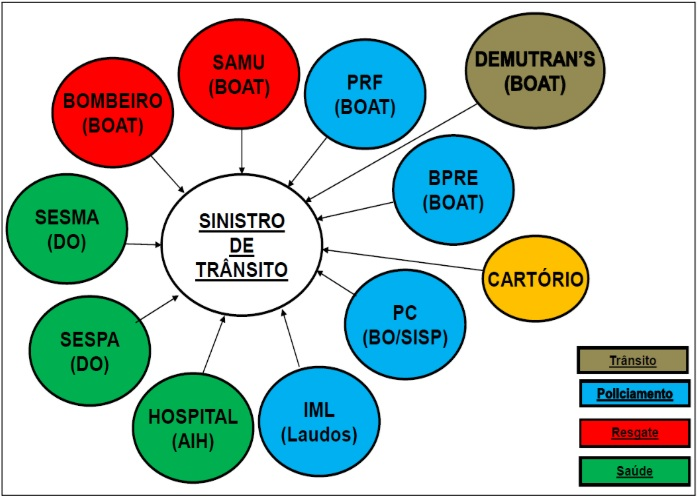
\includegraphics[width=0.95\linewidth]{Tipificacao_sinistro.jpg}
  \caption{Tipificação e Mapeamento das Fontes de Dados sobre Sinistros de Trânsito no Estado do Pará.}
  \label{fig:placeholder}
\end{figure}

A primeira etapa correspondeu ao \textbf{Diagnóstico Situacional}, mapeando as instituições custodiantes e categorizando a natureza do registro: cena imediata, transporte pré-hospitalar, internação clínica ou vigilância de mortalidade. 

A segunda etapa compreendeu a \textbf{Limpeza e Padronização}, responsável por sanar redundâncias sintáticas nos atributos comuns (nome, sexo, idade e logradouro). 

A terceira etapa consistiu na execução do \textbf{Pareamento Probabilístico} (Figura \ref{fig:LUVF1}), convergindo primeiramente as fontes de fiscalização e segurança pública para a consolidação da Lista Única de Vítimas Fatais de Policiamento (LUVF1).

\begin{figure}[htbp]
  \centering
  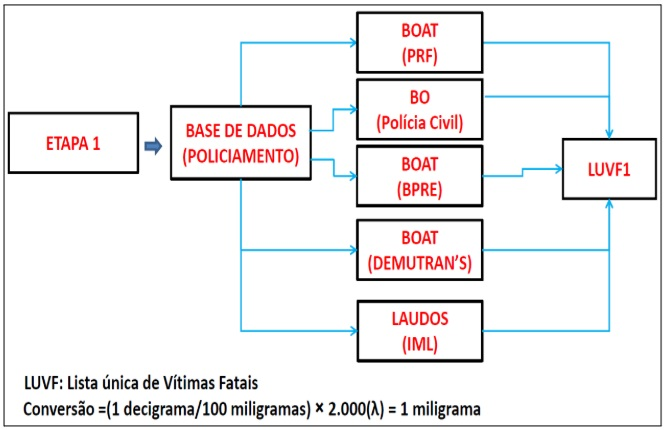
\includegraphics[width=0.95\linewidth]{LUVF_ETAPA1.jpg}
  \caption{Etapa I: Consolidação da Base de Policiamento e Perícia Forense (LUVF1).}
  \label{fig:LUVF1}
\end{figure}

A base $dataset1.csv$ (PRF) e a base $dataset2.csv$ (Polícia Civil) foram unificadas aos dados de laudos periciais toxicológicos do IML e aos boletins digitalizados do BPRE. A incorporação dos dados do IML agregou variáveis de dosagem alcoólica e triagem toxicológica que não constam dos boletins de pista, enriquecendo o potencial investigativo das causas basais dos sinistros.

\begin{figure}[htbp]
  \centering
  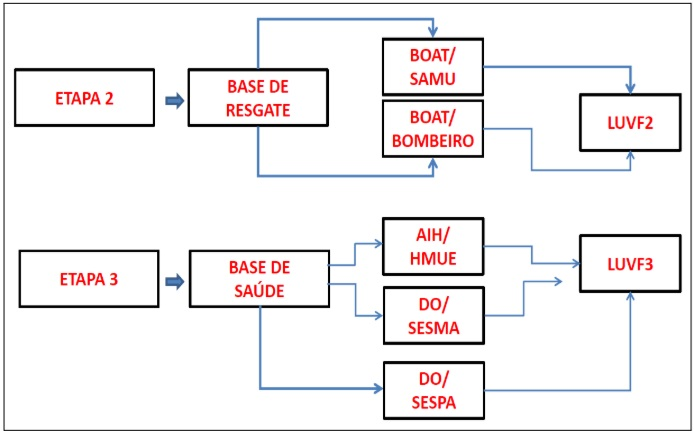
\includegraphics[width=0.95\linewidth]{LUVF_ETAPA2.jpg}
  \caption{Etapas II e III: Integração das Bases de Resgate Pré-Hospitalar e Saúde (LUVF2 e LUVF3).}
  \label{fig:LUVF2}
\end{figure}

Conforme apresentado na Figura \ref{fig:LUVF2}, as Etapas 2 e 3 expandiram a consolidação para o escopo assistencial. Na Etapa 2, o pareamento dos atendimentos do SAMU (\texttt{dataset\_samu.csv}) e do Corpo de Bombeiros (\texttt{dataset\_bombeiro.csv}) gerou a LUVF2, documentando parâmetros de trauma e encaminhamento. Na Etapa 3, a convergência das AIH do SIH/SUS com as Declarações de Óbito (DO) da SESMA e da SESPA estruturou a LUVF3, viabilizando o monitoramento do óbito decorrente do trauma mesmo após dias de internação.

\begin{figure}[htbp]
  \centering
  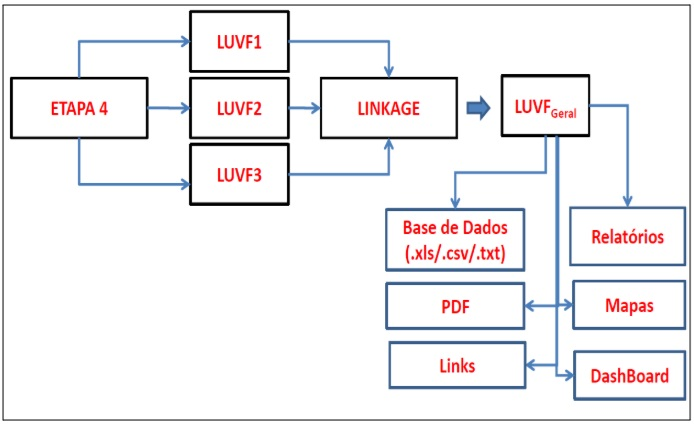
\includegraphics[width=0.95\linewidth]{LUVF_ETAPA3.jpg}
  \caption{Etapa IV: Síntese pelo Módulo de Linkage Central, Formação da LUVF Geral e Camadas de Saída.}
  \label{fig:LUVF3}
\end{figure}

A convergência hierárquica das listas parciais (LUVF1, LUVF2 e LUVF3) no módulo central de linkage culminou na \textbf{Lista Única de Vítimas Fatais Geral (LUVF Geral)}, como ilustrado na Figura \ref{fig:LUVF3}. O relacionamento identificou indivíduos registrados em múltiplos sistemas (ex.: atendimento pré-hospitalar, boletim e declaração de óbito), expurgando duplicidades e gerando uma visão transetorial da vítima. 

A base unificada alimenta múltiplos canais de saída em conformidade com as premissas de dados abertos e reprodutíveis \cite{wilkinson2016}, destacando-se relatórios corporativos, arquivos tabulares e a plataforma analítica interativa.

\begin{figure}[htbp]
  \centering
  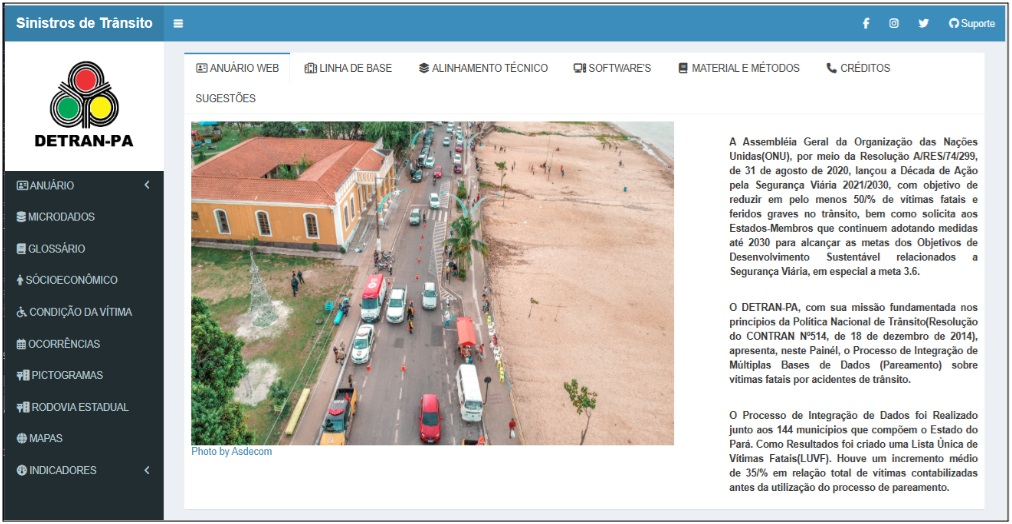
\includegraphics[width=0.95\linewidth]{dahboard1.jpg}
  \caption{Painel Principal do Dashboard de Sinistros de Trânsito Desenvolvido em R/Shiny.}
  \label{fig:aba1_dashboard}
\end{figure}

A aplicação analítica concebida em Shiny está estruturada em abas funcionais. A tela principal (Figura \ref{fig:aba1_dashboard}) sintetiza os indicadores macro da segurança viária estadual, permitindo a filtragem dinâmica por período, região de integração e perfil sociodemográfico (sexo, faixa etária e escolaridade). A combinação do \texttt{echarts4r} e \texttt{leaflet} permite alternar com fluidez entre a visão temporal de tendências e a distribuição territorial da severidade dos eventos.

\begin{figure}[htbp]
  \centering
  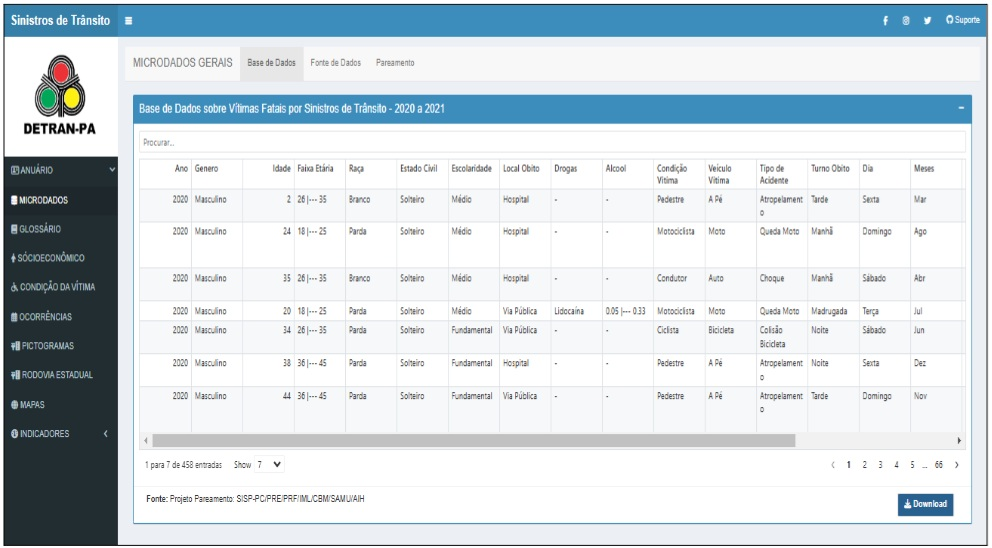
\includegraphics[width=0.95\linewidth]{dahboard2.jpg}
  \caption{Aba de Microdados Dinâmicos com Filtros Multivariados e Exportação via Pacote DT.}
  \label{fig:aba2_microdados}
\end{figure}

A interface de microdados (Figura \ref{fig:aba2_microdados}) disponibiliza o repositório desagregado via tabelas reativas (\texttt{DT}). Usuários técnicos e gestores podem efetuar buscas textuais diretas, reordenar vetores por gravidade e extrair recortes sob demanda para auditorias operacionais.

A aba de distribuição espacial \ref{fig:aba3_microdados} foi construída de modo a permitir que os usuários consigam visualizar o comportamento no espaço dos diferentes sinistros de trânsito, incluídos no painel por meio de mapas coropléticos. Os filtros permitem delimitar o período(ano) e o nível de divisão espacial entre municípios, e os tipos de região de integração.

\begin{figure}[htbp]
  \centering
  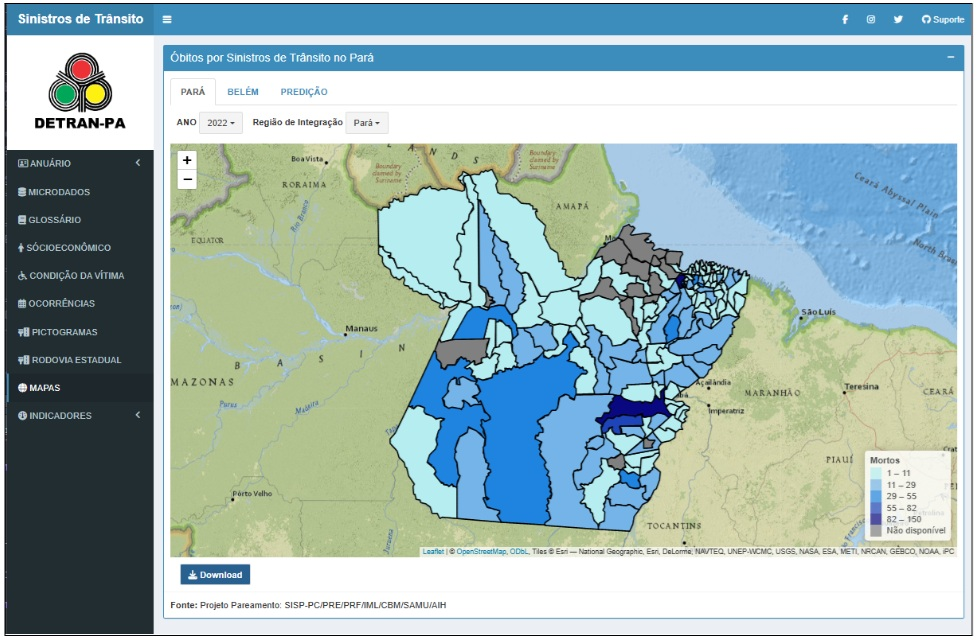
\includegraphics[width=0.95\linewidth]{dahboard3.jpg}
  \caption{Aba referente a distribuição Espacial do Painel de Sinistros de Trânsito criado no framework shiny R}
  \label{fig:aba3_microdados}
\end{figure}

\newpage
O último item do menu é referente aos indicadores, detalhando sobre as principais taxas de mortalidade por sinistros de trânsito. A figura  ilustra as taxas de mortalidade por 100 mil habitantes na condição geral e motociclista.


\begin{figure}[htbp]
  \centering
  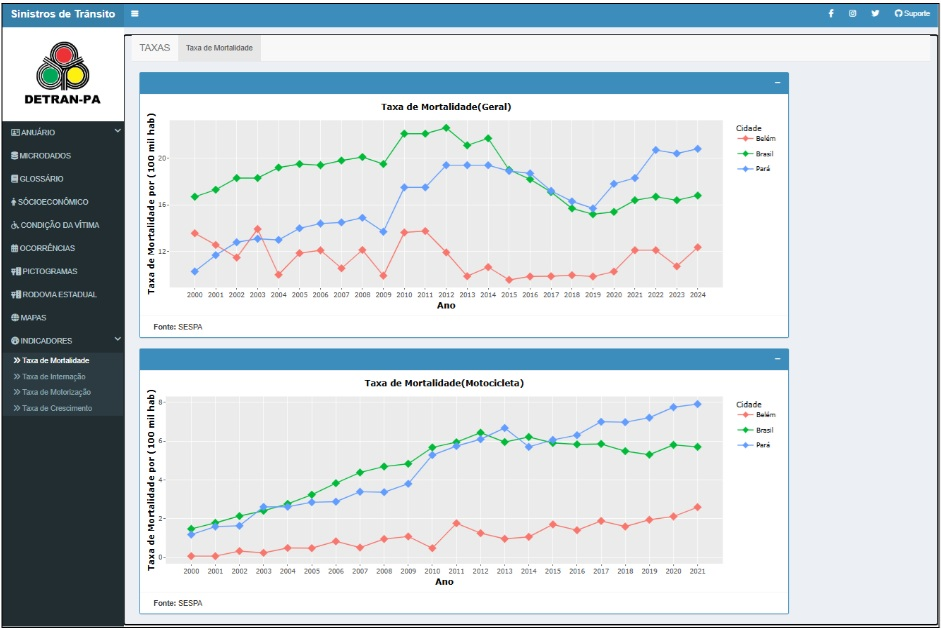
\includegraphics[width=0.95\linewidth]{dahboard4.jpg}
  \caption{ Aba referente aos Indicadores (taxas) do Painel de Sinistros de Trânsito criado no framework shiny R}
  \label{fig:aba4_microdados}
\end{figure}
















%% =====================================================================
%% 5. DISCUSSAO
%% =====================================================================
\section{Discussão}\label{sec:discussao}
A integração multidomínio demonstrou a insuficiência de utilizar exclusivamente as bases de policiamento para dimensionar a mortalidade viária. Vítimas socorridas sem a presença da autoridade policial na pista ou que evoluem a óbito em ambiente hospitalar tendem a ficar ocultas dos sistemas de trânsito convencionais. O pareamento com os registros do SIM e SIH/SUS saneou parcela expressiva do sub-registro histórico, alinhando as estatísticas do estado às diretrizes internacionais \cite{who2018}.

O uso do ecossistema R/Shiny evidenciou vantagens arquiteturais frente às soluções proprietárias anteriores (SPSS e Excel). A capacidade de acoplar rotinas analíticas diretamente ao ambiente de apresentação web viabilizou atualização transparente e automatizada, mitigando inconsistências de integridade manual. Adicionalmente, o design pautado na clareza visual e interatividade atende aos preceitos da visualização de dados para tomada de decisão \cite{few2013}, tornando a informação acessível tanto para gestores quanto para o cidadão comum.

Contudo, a persistência de registros físicos nos postos do BPRE e a ausência de integração sistemática dos dados dos Departamentos Municipais de Trânsito (DEMUTRANs) impõem limites à cobertura em perímetros urbanos interioranos. Esse cenário reforça a necessidade de modernização tecnológica das esferas municipais para viabilizar um inventário censitário do tráfego.

%% =====================================================================
%% 6. CONCLUSAO E TRABALHOS FUTUROS
%% =====================================================================
\section{Conclusões}\label{sec:conclusao}
Este trabalho apresentou o processo de engenharia de dados e desenvolvimento analítico adotado no DETRAN-PA para consolidação das estatísticas de segurança viária. A aplicação do método de Fellegi e Sunter comprovou-se viável e eficaz para a harmonização de bases fragmentadas, culminando na Lista Única de Vítimas Fatais (LUVF Geral). 

A construção do painel em R/Shiny conferiu transparência ativa e providenciou aos gestores públicos uma ferramenta para fiscalização direcionada e formulação de políticas preventivas orientadas por dados.

\subsection{Trabalhos Futuros}\label{sec:trabalhos_futuros}
Como perspectivas de evolução deste trabalho, destacam-se:
\begin{enumerate}
    \item Implementação de algoritmos de aprendizagem de máquina para o refinamento do cálculo dos pesos de pareamento (\textit{active learning});
    \item Integração de rotinas de Extração Automática de Entidades (NER) e Processamento de Linguagem Natural (PLN) para leitura dos relatos narrativos contidos nos boletins de ocorrência;
    \item Expansão da infraestrutura com barramento de APIs REST para recepção de dados em tempo real dos DEMUTRANs;
    \item Incorporação de módulos preditivos de concentração espaço-temporal de sinistros (\textit{hotspot forecasting}) diretamente na interface do Shiny.
\end{enumerate}

%% =====================================================================
%% AGRADECIMENTOS
%% =====================================================================
\begin{acks}
Os autores expressam seus agradecimentos às equipes técnicas da Gerência de Estatística e da Coordenadoria de Planejamento do Departamento de Trânsito do Estado do Pará (DETRAN-PA), bem como aos órgãos parceiros da Segurança Pública e da Saúde do Estado do Pará pelo fornecimento das bases de microdados.
\end{acks}

%% =====================================================================
%% DECLARACAO DE USO DE IA
%% =====================================================================
\section*{Declaração de Uso de Inteligência Artificial}
Durante a preparação deste trabalho, os autores utilizaram ferramentas de Modelos de Linguagem de Grande Porte (LLM) exclusivamente para fins de revisão gramatical, adequação ao padrão de estilo acadêmico e refatoração do código LaTeX. Os autores revisaram criticamente o conteúdo gerado e assumem integral responsabilidade pela integridade e veracidade do manuscrito.

%% =====================================================================
%% REFERENCIAS BIBLIOGRAFICAS
%% =====================================================================
\bibliographystyle{ACM-Reference-Format}
\begin{thebibliography}{99}

\bibitem{batini2016}
C.~Batini and M.~Scannapieco. 2016.
\newblock {\em Data and Information Quality: Dimensions, Principles and Techniques}.
\newblock Springer.

\bibitem{brasil2011}
BRASIL. 2011.
\newblock {\em Manual de instruções para o preenchimento da Declaração de Óbito}.
\newblock Ministério da Saúde, Brasília.

\bibitem{chang2024}
W.~Chang, J.~Cheng, J.~Allaire, C.~Sievert, B.~Schloerke, Y.~Xie, J.~Allen, J.~McPherson, A.~Dipert, and B.~Borges. 2024.
\newblock {\em shiny: Web Application Framework for R}.
\newblock R package version 1.9.1, \url{https://CRAN.R-project.org/package=shiny}.

\bibitem{christen2012}
P.~Christen. 2012.
\newblock {\em Data Matching: Concepts and Techniques for Record Linkage, Entity Resolution, and Duplicate Detection}.
\newblock Springer Science \& Business Media.

\bibitem{echarts4r2023}
J.~Coene. 2023.
\newblock {\em echarts4r: Create Interactive Web Charts with the JavaScript ECharts Library}.
\newblock R package version 0.4.5, \url{https://CRAN.R-project.org/package=echarts4r}.

\bibitem{detran2024}
DETRAN-PA. 2024.
\newblock {\em Anuário Estatístico de Trânsito do Estado do Pará}.
\newblock Departamento de Trânsito do Estado do Pará, Belém.

\bibitem{doan2012}
A.~Doan, A.~Halevy, and Z.~Ives. 2012.
\newblock {\em Principles of Data Integration}.
\newblock Morgan Kaufmann.

\bibitem{elvik2004}
R.~Elvik and T.~Vaa. 2004.
\newblock {\em The Handbook of Road Safety Measures}.
\newblock Elsevier.

\bibitem{fellegi1969}
I.~P. Fellegi and A.~B. Sunter. 1969.
\newblock A theory for record linkage.
\newblock {\em Journal of the American Statistical Association} 64, 328 (1969), 1183--1210.

\bibitem{few2013}
S.~Few. 2013.
\newblock {\em Information Dashboard Design: Displaying Data for At-a-Glance Monitoring} (2nd ed.).
\newblock Analytics Press.

\bibitem{ibm2020}
IBM~Corp. 2020.
\newblock {\em IBM SPSS Statistics for Windows, Version 27.0}.
\newblock IBM Corp, Armonk, NY.

\bibitem{lenzerini2002}
M.~Lenzerini. 2002.
\newblock Data integration: A theoretical perspective.
\newblock In {\em Proceedings of the twenty-first ACM SIGMOD-SIGACT-SIGART symposium on Principles of database systems}. ACM, 233--246.

\bibitem{mellojorge2007}
M.~H.~P. Mello~Jorge, R.~Laurenti, and S.~L.~D. Gotlieb. 2007.
\newblock Análise da qualidade das estatísticas vitais brasileiras: a experiência de implantação do SINASC e do SIM.
\newblock {\em Ciência \& Saúde Coletiva} 12, 3 (2007), 643--654.

\bibitem{rahm2000}
E.~Rahm and H.~H. Do. 2000.
\newblock Data cleaning: Problems and current approaches.
\newblock {\em IEEE Data Engineering Bulletin} 23, 4 (2000), 3--13.

\bibitem{rcore2024}
R~Core~Team. 2024.
\newblock {\em R: A Language and Environment for Statistical Computing}.
\newblock R Foundation for Statistical Computing, Vienna, Austria. \url{https://www.R-project.org/}.

\bibitem{veras1994}
C.~M.~T. Veras and M.~S. Martins. 1994.
\newblock A confiabilidade dos dados nos formulários de Autorização de Internação Hospitalar (AIH).
\newblock {\em Cadernos de Saúde Pública} 10, 3 (1994), 339--355.

\bibitem{who2018}
WHO. 2018.
\newblock {\em Global Status Report on Road Safety 2018}.
\newblock World Health Organization, Geneva.

\bibitem{wilkinson2016}
M.~D. Wilkinson et~al. 2016.
\newblock The FAIR Guiding Principles for scientific data management and stewardship.
\newblock {\em Scientific Data} 3 (2016), 160018.

\bibitem{dt2024}
Y.~Xie, J.~Cheng, and X.~Tan. 2024.
\newblock {\em DT: A Wrapper of the JavaScript Library 'DataTables'}.
\newblock R package version 0.33, \url{https://CRAN.R-project.org/package=DT}.

\bibitem{leaflet2024}
J.~Cheng, B.~Karambelkar, and Y.~Xie. 2024.
\newblock {\em leaflet: Create Interactive Web Maps with the JavaScript 'Leaflet' Library}.
\newblock R package version 2.2.2, \url{https://CRAN.R-project.org/package=leaflet}.

\end{thebibliography}
\end{document}